%%%%%%%%%%%%%%%%%%%%%%%%%%%%%%%%%%%%%%%%%%%%%%%%%%%%%%%%%%%%%%%%%%%%%%%%%%%%
% riemann_hibs_zh.tex
%
% 使用 XeLaTeX 编译，然后运行 BibTeX，再运行两次 XeLaTeX。
%
% 论证范围：本文区分经典输入、坐标变换的严格推论与开放命题，
% 不把形式化名称的罗列冒充为黎曼猜想的新证明。
%%%%%%%%%%%%%%%%%%%%%%%%%%%%%%%%%%%%%%%%%%%%%%%%%%%%%%%%%%%%%%%%%%%%%%%%%%%%

\documentclass[submission,noinfoline]{jsfds}
\usepackage{fontspec}
\usepackage{xeCJK}
% 本机优先使用 PingFang；Overleaf 上回退到 Noto 或 Fandol。
\IfFileExists{/System/Library/Fonts/PingFang.ttc}{%
  \setCJKmainfont{PingFang.ttc}[Path=/System/Library/Fonts/]
  \setCJKsansfont{PingFang.ttc}[Path=/System/Library/Fonts/]
  \setCJKmonofont{PingFang.ttc}[Path=/System/Library/Fonts/]
}{%
  \IfFontExistsTF{Noto Serif CJK SC}{%
    \setCJKmainfont{Noto Serif CJK SC}
    \setCJKsansfont{Noto Serif CJK SC}
    \setCJKmonofont{Noto Serif CJK SC}
  }{%
    \setCJKmainfont{FandolSong-Regular.otf}
    \setCJKsansfont{FandolSong-Regular.otf}
    \setCJKmonofont{FandolSong-Regular.otf}
  }%
}
\usepackage{amsmath,amsthm,amssymb}
\usepackage{graphicx}
\usepackage{natbib}
\usepackage{hyperref}
\makeatletter\let\hy@frontmatter\relax\makeatother
\setlength{\emergencystretch}{2em}

\graphicspath{{figures/}}

\startlocaldefs
\newtheorem{theorem}{定理}
\newtheorem{proposition}[theorem]{命题}
\newtheorem{corollary}[theorem]{推论}
\newtheorem{lemma}[theorem]{引理}
\newtheorem{definition}[theorem]{定义}
\newtheorem*{remark}{注}
\setattribute{title}{size}{\LARGE\bfseries}
% Lean 名字保留在源码中作为交叉引用，但不显示在成稿中。
\newcommand{\Lean}[1]{}
\def\journal@name{}%
\setattribute{infoline}{text}{}%
\setattribute{copyright}{text}{}
\newcommand{\abs}[1]{\lvert #1\rvert}
\newcommand{\Norm}[1]{\lVert #1\rVert}
\endlocaldefs

\setmainlanguageenglish
\makeatletter
\def\abstractname{摘要}%
\addto\captionsenglish{%
  \def\abstractname{摘要}%
  \def\jsfds@kwname{关键词：}%
  \def\jsfds@AMSname{AMS 2000 学科分类：}%
}
\makeatother
\firstpage{1}
\begin{document}
\begin{frontmatter}

\title{临界圆上的黎曼 \texorpdfstring{$\zeta$}{zeta} 函数：
从经典输入到隐数坐标约化}
\runtitle{从经典输入到临界圆约化}

\begin{aug}
  \auteur{%
    \prenom{Yuanjie}
    \nom{Liu}}
  \affiliation{独立研究者；\quad
  \href{mailto:yuanjieliu65@gmail.com}{yuanjieliu65@gmail.com}}
  \runauthor{Yuanjie Liu}
\end{aug}

\begin{abstract}
本文从数学论证的依赖关系出发，重新组织隐数坐标系下的黎曼
$\zeta$ 函数。本文使用的隐数空间，是作者在前期工作中提出并发展的
坐标框架 \citep{LiuXu2026bridge}；本篇在这一既有构造上研究 $\zeta$ 的零点。
先把函数方程、零域半平面和 Hardy 的临界线零点定理作为
经典输入；再由变换 $w=e^s$ 严格推出反射 $s\mapsto1-s$ 对应反演
$w\mapsto e/w$，并推出临界线对应唯一的不动圆 $|w|=\sqrt e$。于是，
非平凡零点落在圆环 $1<|w|<e$，并按反射成对出现；Hardy 定理则直接传输为
临界圆上方的提升零点有无限多个。这是已知定理的坐标化，而不是 Hardy 定理或黎曼猜想
的新证明。能量与频率计算作为严格的坐标诊断附后：它们说明 $1/2$ 的尺度和
有限近似的频率结构，但不能单独产生零点或证明密度公式。最后，黎曼猜想被
明确隔离为：圆环中的每个反射对都必须是自配对。Lean 标识符保留在源码中
便于追溯，但不出现在成稿中。
\end{abstract}

\begin{keywords}
\kwd{黎曼猜想}
\kwd{黎曼 zeta 函数}
\kwd{隐数坐标系}
\kwd{临界圆}
\kwd{形式化验证}
\end{keywords}

\begin{AMSclass}
\kwd{11M26}
\kwd{11A25}
\kwd{03B35}
\end{AMSclass}
\end{frontmatter}

\section{问题、输入与论证顺序}\label{sec:intro}

黎曼猜想研究 $\zeta(s)$ 的非平凡零点，断言
\[
  0<\Re s<1,\quad \zeta(s)=0
  \quad\Longrightarrow\quad \Re s=\tfrac12 .
\]
本文的目标不是把形式化对象逐个堆叠，而是把“已知什么、由此推出什么、
还缺什么”写成一条可检查的推导链。全文使用三类陈述：

\begin{description}
\item[经典输入。] 函数方程、标准零域结果以及 Hardy 定理作为已知的分析定理。
\item[严格推论。] 坐标变换、模长恒等式、反射配对，以及临界线与临界圆的
等价描述直接由定义和上述输入推出。
\item[开放命题。] 圆环中不存在非自配对零点正是黎曼猜想。数值密度和能量
启发不能用来遮蔽这一步缺口。
\end{description}

\paragraph{文献背景。}
黎曼的原始工作是这一理论的奠基文献 \citep{Riemann1859}。关于零点分布
及其与素数计数的关系，可参见 von Mangoldt、Hadamard 和 de la Vall{\'e}e
Poussin 的经典工作 \citep{vonMangoldt1905,Hadamard1893,
deLaValleePoussin1899}；von Koch、Schoenfeld 和 Lagarias 讨论了若干等价的
初等表述 \citep{vonKoch1901,Schoenfeld1976,Lagarias2002}。下文所需的
临界线零点存在性输入来自 Hardy 定理 \citep{Hardy1914}，其后的定量发展
包括 Hardy--Littlewood、Selberg、Levinson、Heath-Brown 与 Conrey 的工作
\citep{HardyLittlewood1921,Selberg1942,Levinson1974,HeathBrown1979,
Conrey1989}。Montgomery 的对相关研究以及 Connes、Bombieri--Hejhal 的
谱观点提供了进一步背景 \citep{Montgomery1973,Montgomery1977,
Connes1999,BombieriHejhal1995}；Platt 和 Trudgian 给出了很高高度的
有限数值验证 \citep{PlattTrudgian2021}。标准专著与综述包括 Edwards、
Titchmarsh、Iwaniec--Kowalski、Iwaniec 和 Conrey
\citep{Edwards1974,Titchmarsh1986,IwaniecKowalski2004,Iwaniec2014,
Conrey2003}。

因此下文依次处理：坐标字典、反射强制的候选圆、零点的圆环定位与配对、
Hardy 定理的直接传输，最后才讨论能量/频率诊断及尚未解决的问题。

这样的顺序是有意安排的。$s$ 平面是陈述 $\zeta$ 经典分析事实的地方，
而 $w$ 平面使反射几何变得透明。因此，本文不从“坐标能否制造一个零点”
开始，而是先说明坐标变换保留了什么，再把它应用于零点集已有的性质，最后
讨论有限和与数值实验能够提供什么。这样可以避免把几何图像误读成解析的
零点计数论证。

\section{坐标字典}\label{sec:coords}

\paragraph{空间来源与本文贡献。}
隐数空间并不是本文为了书写方便临时引入的记号，而是作者在前期工作中提出并
发展的坐标框架 \citep{LiuXu2026bridge}。它的基本思想是同时保留半径坐标和
提升后的角坐标：投影到穿孔平面 $w\neq0$ 时叶编号会被遗忘，而在对数覆盖中
叶编号仍被保留。这样，$s$ 平面中的竖直平移就可以被记录为同一个穿孔平面点
上不同提升之间的运动。因而，本篇的贡献边界是明确的：在作者已有的隐数空间
构造上整理 $\zeta$ 零点的论证，推出反射与反演的对应关系，并把严格的坐标推论、
经典分析输入以及尚未解决的开放命题分开。

写 $s=\sigma+it$，定义
\[
  \Phi(s)=e^s=w=e^\sigma e^{it}.
\]
半径记录实部，辐角只记录模 $2\pi$ 的虚部。因此自然的定义域是对数覆盖：
一个点同时记住 $w\neq0$ 和叶编号。这只是坐标变换，不是对 $\zeta$ 增加的新假设。

\begin{definition}[隐数坐标]\label{def:coords}
$s=\sigma+it$ 的隐数坐标是 $(w,k)$，其中 $w=e^s$，而 $k$ 记录 $t$
在模 $2\pi$ 意义下的提升。特别地，
\[
  |w|=e^\sigma,\qquad \log|w|=\sigma .
\]
\end{definition}

更具体地，取 $\theta\in[0,2\pi)$ 和叶编号 $k\in\mathbb Z$，对数覆盖中的
一点可以写成
\[
  w=re^{i\theta},\qquad
  s=\log r+i(\theta+2\pi k),\qquad r>0.
\]
投影会忘记 $k$，因为所有这些提升都投影到同一个 $w$；但覆盖空间不会把
相应的 $s$ 识别为同一点：改变 $k$ 就把高度改变 $2\pi$，从而得到楼上的
另一个点。这正是隐数空间保留而穿孔 $w$ 平面看不见的信息。它也说明，
隐数空间并没有把 $\zeta$ 换成另一个函数；我们仍然在提升点 $s$ 处计算
$\zeta$，只是用另一种方式保存径向和角向数据。

对移位后的 Dirichlet 项，同样的分解是
\[
  (n+1)^{-s}=(n+1)^{-\sigma}
  \exp\bigl(-it\log(n+1)\bigr).
\]
第一因子是径向数据，第二因子是提升后的角向数据。这个初等恒等式说明，
后文的能量与频率计算为什么适合放在几何约化之后：它们分别观察两个坐标，
但还没有对解析延拓作出任何结论。

函数方程把 $s$ 反射到 $1-s$。在 $\Phi$ 下，
\[
  \Phi(1-s)=e^{1-s}=\frac{e}{e^s}=\frac{e}{w},
\]
即得到严格的对应
\[
  s\longmapsto1-s
  \qquad\Longleftrightarrow\qquad
  w\longmapsto\iota(w):=\frac ew .
\]

\begin{figure}[t]
\centering
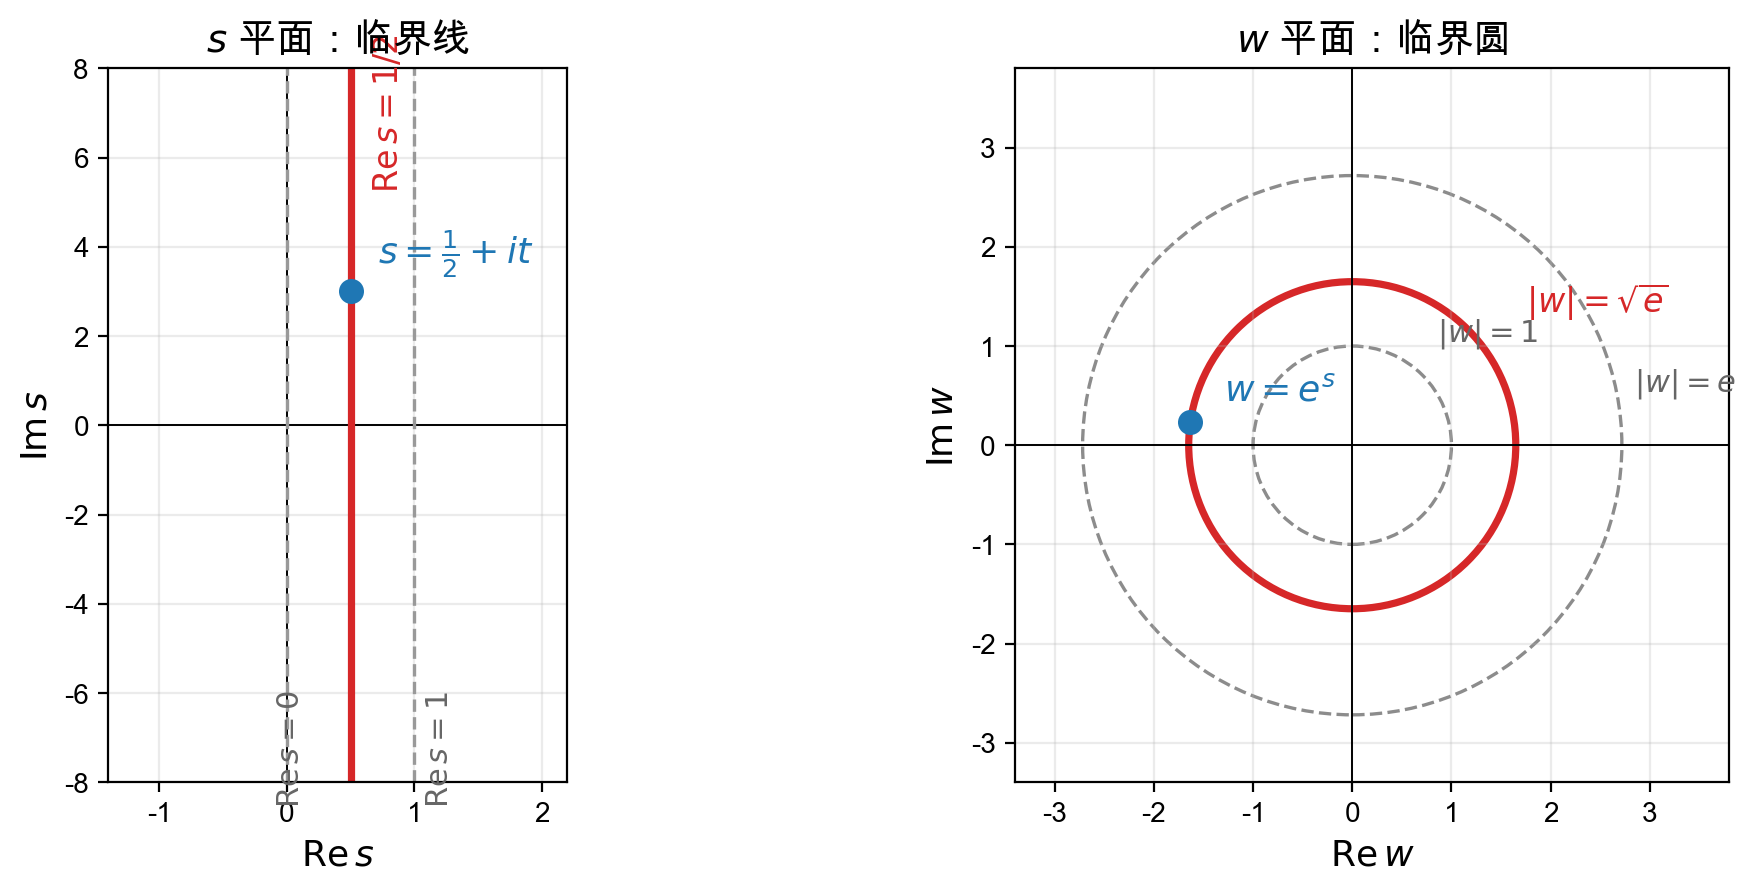
\includegraphics[width=0.85\textwidth]{fig1_projection_cross_zh}
\caption{坐标投影 $w=e^s$。直线 $\Re s=\sigma$ 变为圆 $|w|=e^\sigma$，
临界线变为 $|w|=\sqrt e$。}
\label{fig:proj}
\end{figure}

\section{由反射推出候选临界圆}\label{sec:crit}

先讨论几何，不讨论零点。对任意实数 $t$，
\[
  \left|e^{1/2+it}\right|=e^{1/2}=\sqrt e .
\]

\begin{theorem}[临界线映为圆]\label{thm:critcircle}
在 $w=e^s$ 下，直线 $\Re s=1/2$ 的像恰为圆 $|w|=\sqrt e$。
\end{theorem}

反演对半径的作用为 $\rho\mapsto e/\rho$，所以被反演保持的圆必须满足
$e/\rho=\rho$。

\begin{proposition}[唯一反演不动圆]\label{prop:fixedcircle}
以原点为中心且被 $\iota(w)=e/w$ 保持的圆只有 $|w|=\sqrt e$；其对数半径为
$\log\sqrt e=1/2$。
\end{proposition}

这里必须区分两种“固定”。从集合意义看，反演把半径为 $\rho$ 的圆送回
同一个圆时，得到的是半径 $\sqrt e$ 的选择；从点意义看，一个具体点还必须
满足 $e/w=w$。前一个条件只选定半径，后一个条件只选出两个点
$w=\pm\sqrt e$。所以临界圆是自反射的唯一几何候选，并不意味着圆上每一点
都被逐点固定，更不意味着圆上每一点都是零点。

\begin{remark}[几何身份不等于零点存在]\label{rem:twolayers}
该命题只确定了自反射可能发生的圆，不说明 $\zeta$ 在圆上有零点。零点的
存在性与丰度是另一个分析问题，下面用 Hardy 的经典定理处理。
\end{remark}

\begin{figure}[t]
\centering
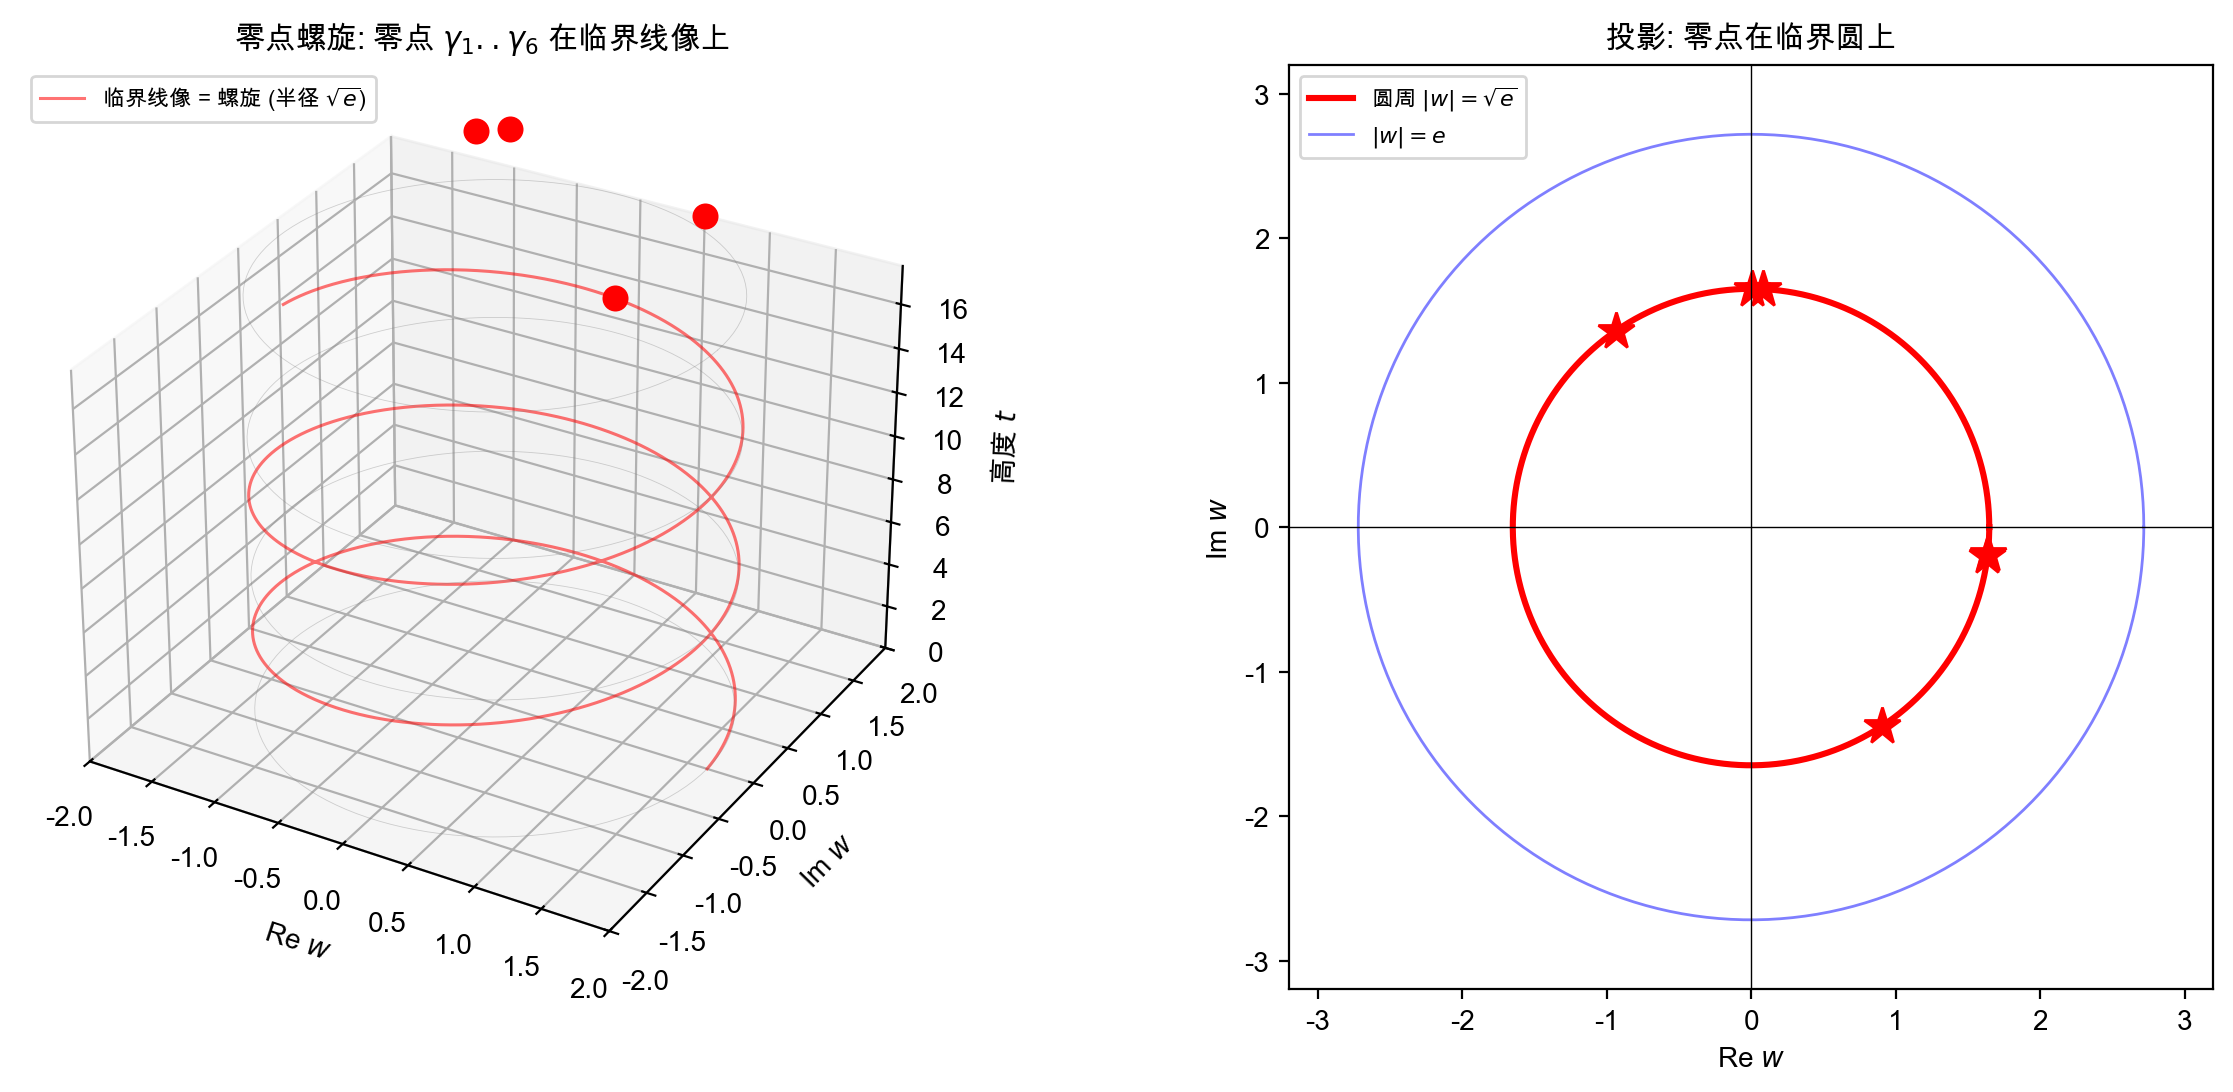
\includegraphics[width=0.85\textwidth]{fig8_static_zh}
\caption{对数覆盖的静态图像。临界线提升为半径 $\sqrt e$ 的螺旋，并投影到
临界圆。}
\label{fig:cover}
\end{figure}

\section{经典零点信息给出的定位与配对}\label{sec:localization}

现在加入关于 $\zeta$ 的已知信息，并沿着黎曼猜想所需的方向推导。欧拉乘积
给出 $\Re s\geq1$ 的标准零域；函数方程与平凡零点处理另一侧。因此非平凡零点
满足
\[
  \zeta(s)=0\ \text{且 $s$ 非平凡}
  \quad\Longrightarrow\quad 0<\Re s<1.
\]
由 $|w|=e^{\Re s}$，这在隐数坐标中就是
\[
  1<|w|<e.
\]

这里的严格不等式很重要。外边界 $|w|=e$ 对应 $\Re s=1$，通常由 Euler
乘积给出零点自由性；内边界 $|w|=1$ 对应 $\Re s=0$，在分离平凡零点和
函数方程中的特殊点后，非平凡零点被限制在开临界带内。因此，坐标变换把
经典的开带结论搬运成开圆环结论，但它本身并没有加强经典零域结果。

\begin{theorem}[反射配对]\label{thm:reflect}
若 $0<\Re s<1$ 且 $\zeta(s)=0$，则 $\zeta(1-s)=0$，反之亦然。在隐数坐标
中，这一对为 $(w,e/w)$。
\end{theorem}

这是函数方程在临界带内的直接推论，其中函数方程的因子均不为零。它说明的
是零点集的对称性，还没有说明一对中的两个零点相同。

从几何上看，偏离候选圆的零点会在圆的另一侧带来一个不同的伴侣。反演
$w\mapsto e/w$ 交换半径 $\rho$ 和 $e/\rho$，并保持它们的乘积为 $e$；只有
$\rho=\sqrt e$ 时两者才相等。因此，函数方程留下的问题不是反射是否存在，
而是零点集是否含有真正的非自配对轨道。

\begin{theorem}[自配对与临界圆]\label{thm:selfpair}
对 $w\neq0$，
\[
  \frac ew=w
  \quad\Longleftrightarrow\quad
  w^2=e
  \quad\Longleftrightarrow\quad
  w=\pm\sqrt e .
\]
因此自配对零点若存在，必在 $|w|=\sqrt e$ 上。
\end{theorem}

于是得到本文的核心约化：

\begin{corollary}[剩余陈述正是黎曼猜想]\label{cor:rh-reduction}
对非平凡零点，黎曼猜想等价于圆环 $1<|w|<e$ 中每个反射对都是自配对；
也等价于不存在偏离 $|w|=\sqrt e$ 的非自配对零点。
\end{corollary}

这只是约化，并不是解答。若从黎曼猜想出发，所有非平凡零点都有
$\Re s=1/2$，于是都落在临界圆上；反过来，若圆环中的每个反射轨道都
坍缩为自配对，前面的代数就强制 $w^2=e$，相应提升满足 $\Re s=1/2$。
两个方向使用的材料不同：前者是原坐标中猜想的定义，后者则使用反射配对
和自配对计算。

\begin{figure}[t]
\centering
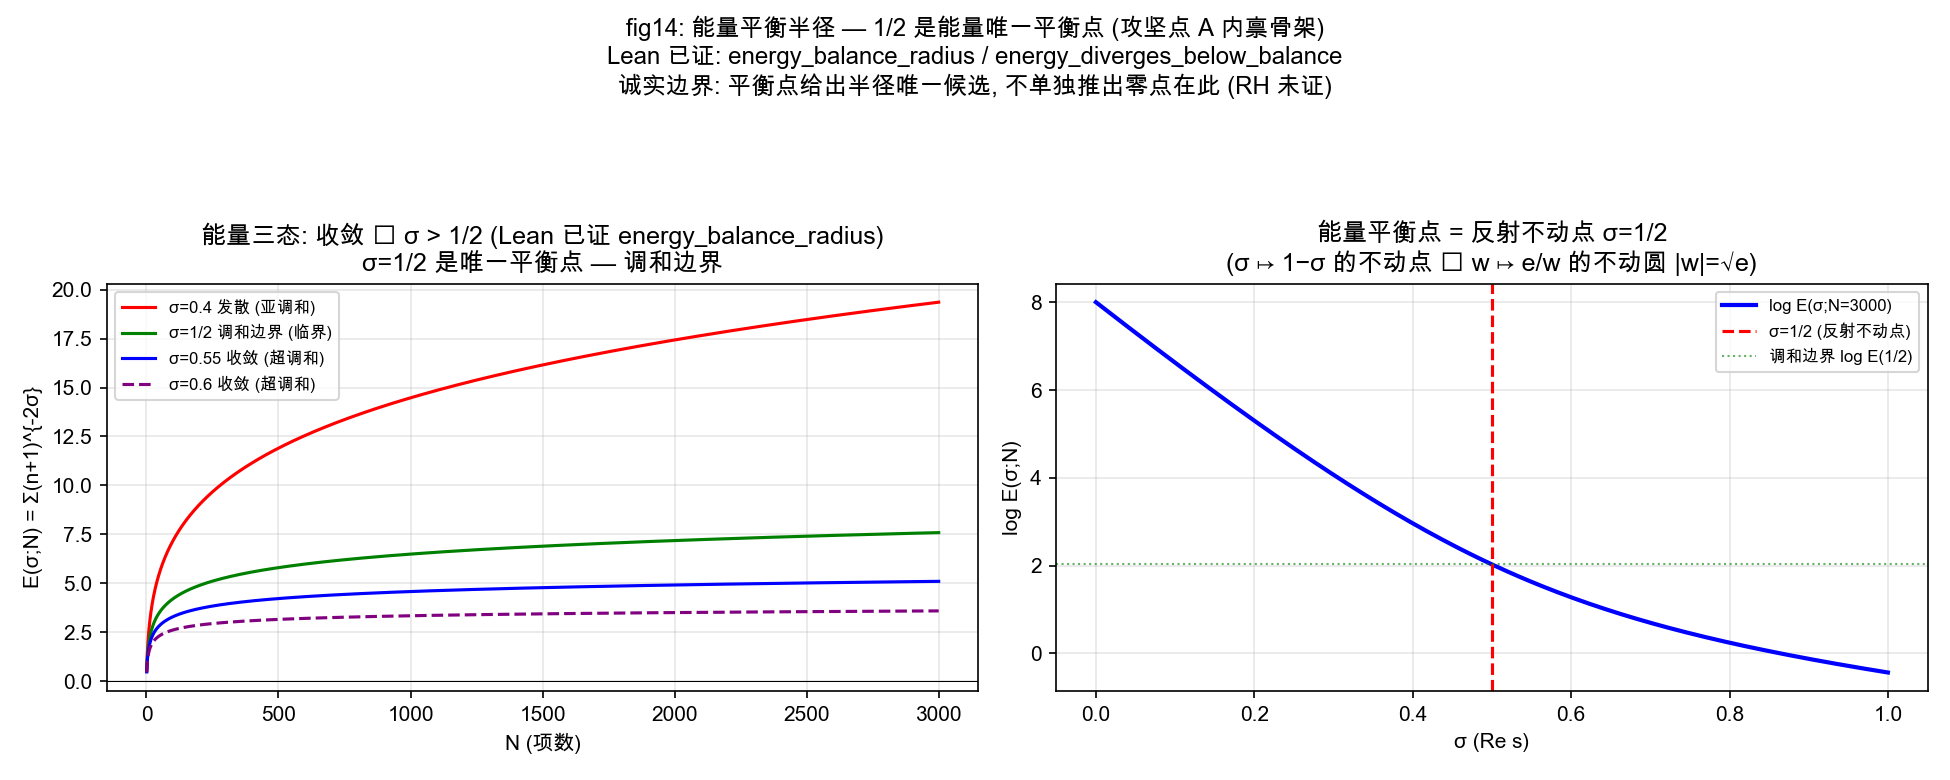
\includegraphics[width=0.85\textwidth]{fig14_zh}
\caption{坐标中的两个尺度：反射不动半径是 $\sqrt e$，而 $\Re s=1$ 的零域边界
对应 $|w|=e$。}
\label{fig:balance}
\end{figure}

\section{圆上丰度：传输 Hardy 的已知定理}\label{sec:abundance}

前面只得到位置约束，尚未产生一个零点。现在使用 Hardy 的经典定理：临界线
上有无限多个 $\zeta$ 的非平凡零点 \citep{Hardy1914}。

\begin{theorem}[Hardy 定理的隐数坐标表述]\label{thm:hardy-transport}
临界圆 $|w|=\sqrt e$ 上方的提升空间中有无限多个 $\zeta$ 零点。
\end{theorem}

\begin{proof}
令 $Z$ 为 Hardy 定理给出的临界线零点无限集。对数覆盖记住提升后的高度；
由定理~\ref{thm:critcircle}，$Z$ 中每个零点都对应于 $|w|=\sqrt e$
上方的一个提升点。因此对应的提升圆上零点集是无限的。
\end{proof}

这是一条传输定理，不是 Hardy 定理的新证明。隐数坐标的正确作用是改变已知
丰度定理的几何语言，同时保留其逻辑内容。

这里“提升”一词很重要。指数映射会把高度按 $2\pi$ 取模，而隐数空间保留
零点所在的叶。因此，Hardy 定理给出的无限零点仍然作为楼上的无限多个对象
被保留下来，即使在投影后它们都只显示同一个半径 $\sqrt e$。投影并没有
制造新的零点；存在性与无限性完全来自 Hardy 定理。

\section{能量与频率诊断}\label{sec:diagnostics}

坐标变换还显露出两个有用的诊断量。它们解释 $1/2$ 的尺度，并描述高度如何
进入有限近似，但不能被提升为零点存在性证明。

Dirichlet 项满足
\[
  (n+1)^{-s}=(n+1)^{-\sigma}
  \exp\bigl(-it\log(n+1)\bigr),
  \qquad
  \bigl|(n+1)^{-s}\bigr|=(n+1)^{-\sigma}.
\]
在临界线上，平方模长为 $(n+1)^{-1}$，故对角能量具有调和尺度
\[
  \sum_{n\leq N}\bigl|(n+1)^{-1/2-it}\bigr|^2
  =\sum_{n\leq N}\frac1{n+1}\sim\log N.
\]
这是关于项和有限和的严格计算，不是临界带内解析延拓后的 $\zeta$ 值估计。

这也是把诊断内容放在零点论证之后的主要原因。在绝对收敛半平面，Dirichlet
级数及其部分和可以用标准极限论证联系起来；但在临界带中，我们研究的是
解析延拓后的函数。有限向量和可以发生抵消，却不必对应 $\zeta$ 的零点；
对角能量发散，也可能和交叉项的大量抵消同时存在。能量计算确定了一个尺度，
却没有补上所缺的解析桥梁。

相邻对数频率满足
\[
  \Delta\mathrm{freq}(n)=\log\frac{n+2}{n+1},\qquad
  \Delta\mathrm{freq}(n)\longrightarrow0,\qquad
  \Delta\mathrm{freq}(n+1)\leq\Delta\mathrm{freq}(n).
\]
交错近似的相位差为
\[
  \Delta\theta_n=\pi-t\,\Delta\mathrm{freq}(n).
\]
当 $t\log2>\pi$ 时，这个单调量变号一次，变号指标的量级为 $t/\pi$。
这些恒等式刻画有限频率骨架，适合组织数值实验。

频率结论同样具有有限但有用的作用。它说明指标增大时，对数频率在局部变得
更接近，所以高高度实验中会出现相邻相位增量很小的长段；这可以提示部分和
可能出现相干运动或折返。但它没有说明运动一定到达原点；即使某个截断和
到达原点，也还需要尾项估计，才能把它识别为 $\zeta$ 的零点。

\begin{figure}[t]
\centering
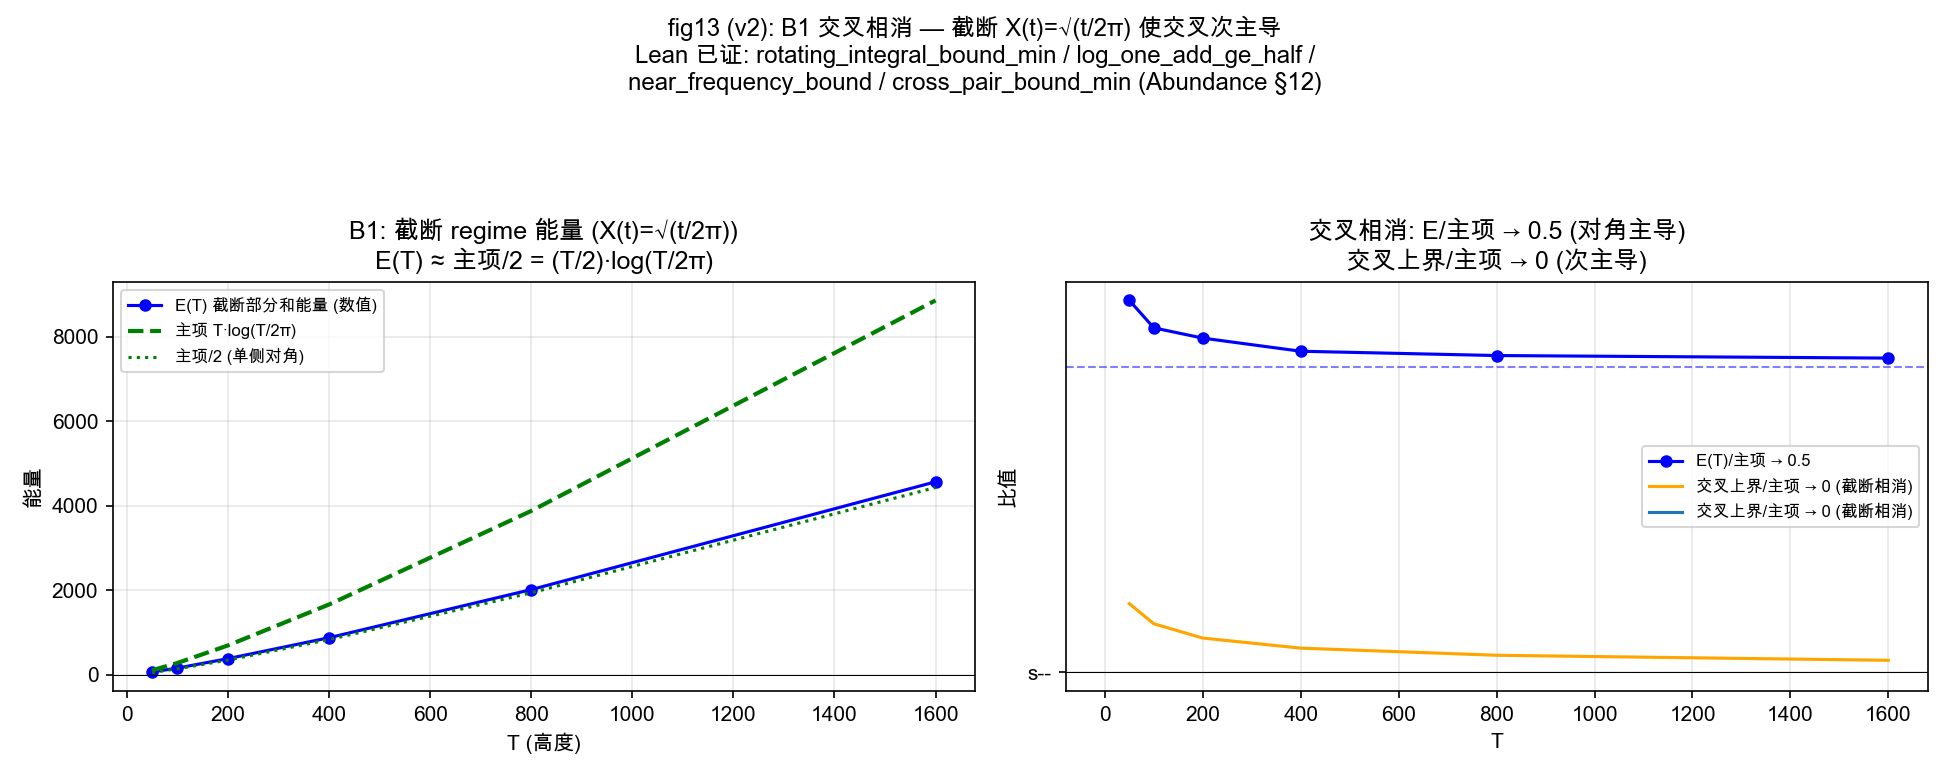
\includegraphics[width=0.85\textwidth]{fig13_zh}
\caption{截断和的数值能量预算。图中展示调和尺度，但它不是零点计数定理的替代品。}
\label{fig:budget}
\end{figure}

\begin{figure}[t]
\centering
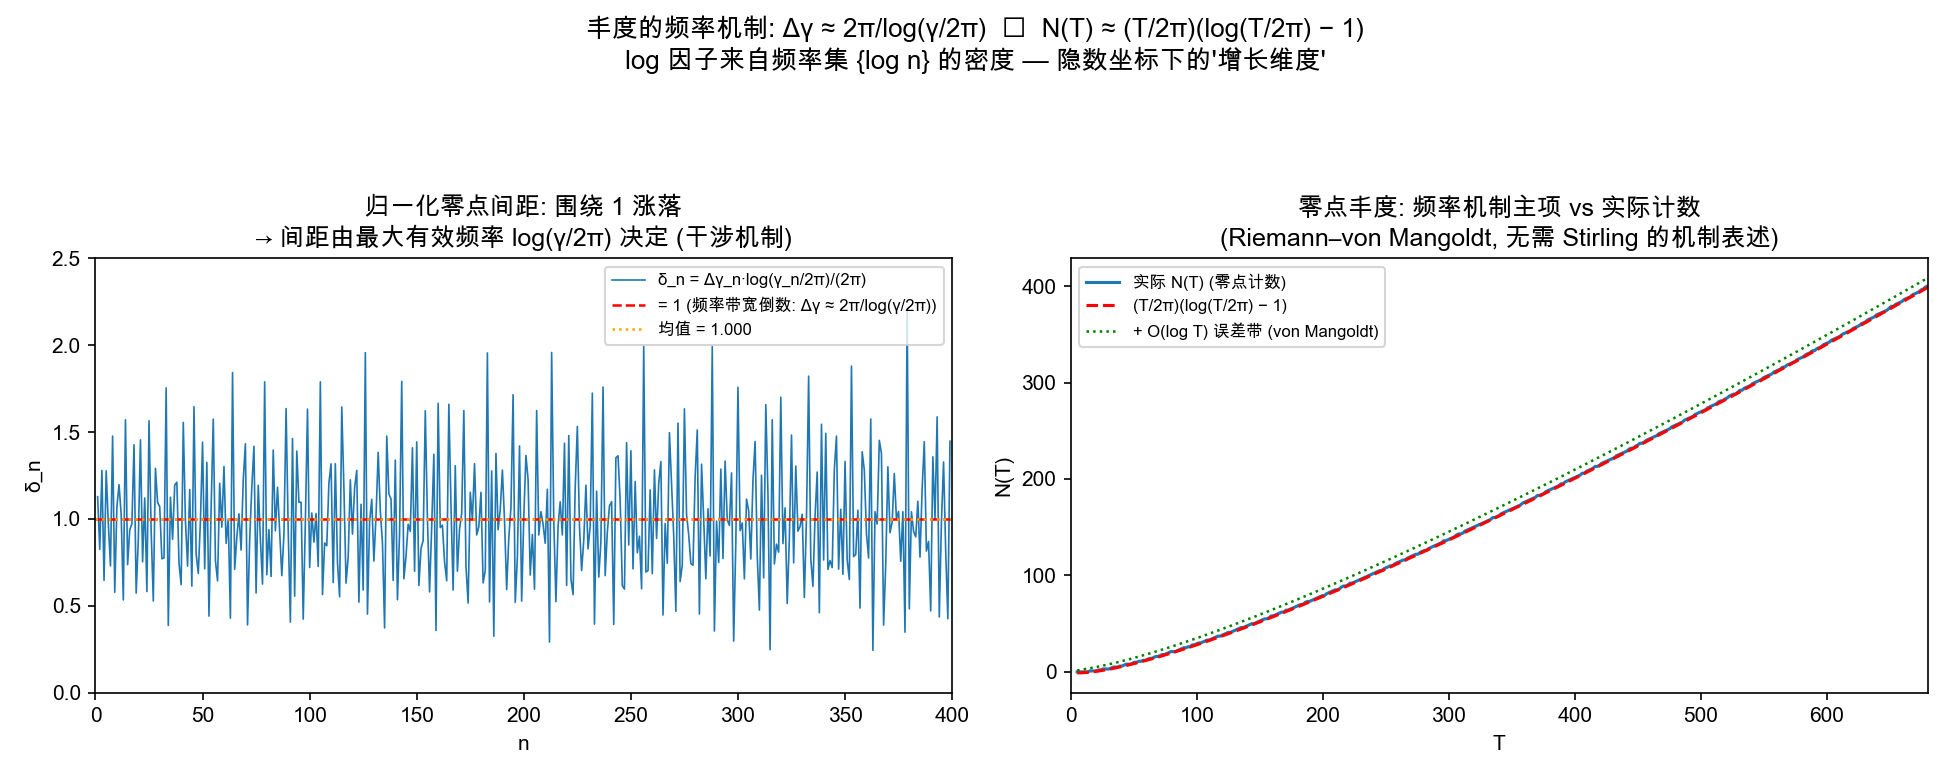
\includegraphics[width=0.85\textwidth]{fig11_zh}
\caption{零点间距与频率的数值诊断。数值比较可以提示密度规律，但不能证明该规律。}
\label{fig:abundance}
\end{figure}

\begin{remark}[诊断为何不能完成 RH]\label{rem:diagnostics}
在临界带内，Dirichlet 级数的有限部分和不能直接等同于解析延拓。有限部分
和出现对齐不等于 $\zeta$ 为零；调和能量发散也不提供零点计数估计。要把它们
接成内部证明，仍需对解析延拓函数建立边界估计，以及幅角原理或零点计数定理。
\end{remark}

\section{形式化记录与论证边界}\label{sec:honesty}

Lean 开发记录了上述许多代数和序理论组件：坐标恒等式、反演、反射 involution、
自配对代数、调和级数与频率引理，以及其适用范围内的初等零域估计。源码仍保留
诸如 \Lean{criticalLine_circle}、\Lean{zeta_zero_iff_one_sub} 和
\Lean{freq_gap_tendsto_zero} 的标识符，但成稿隐藏这些名字以保持数学叙述连贯。

因此，形式化名字应被理解为可追溯层，而不是假设的替代品。关于 $e^s$ 的
定理证明的是坐标恒等式，并不会自动导入 Hardy 定理；描述无界零点族的谓词
记录的是分析输入的形状，也不会自动提供该输入的实例。尤其在最终的黎曼
猜想约化中，保留这些层次差别，才能如实说明剩余命题仍然开放。

本文的推导边界可压缩为四步：

\begin{enumerate}
\item 由 $w=e^s$ 推出临界圆，并解释其对数半径为何是 $1/2$。
\item 由经典零域信息推出临界圆环，由函数方程推出反射配对。
\item 由 Hardy 已知定理直接推出临界圆上有无限多个零点。
\item 圆环中排除非自配对零点仍是开放问题，恰好就是黎曼猜想；坐标变换、
能量计算和频率诊断都没有证明这一步。
\end{enumerate}

如果未来要不用 Hardy 输入而在坐标系内部证明丰度，就必须补上解析延拓的
零点计数或边界绕数估计。明确指出这个要求，本身就是论证的一部分。

\section{结论}\label{sec:conclusion}

隐数坐标 $w=e^s$ 把已知理论组织成一条短的推导链：函数方程反射变为
$w\mapsto e/w$；唯一不动圆是 $|w|=\sqrt e$；标准零域把非平凡零点放入
$1<|w|<e$；函数方程使其成反射对；Hardy 定理则给出圆上方提升空间中的无限多个零点。
剩余的偏离临界圆排除正是黎曼猜想。能量与频率结构澄清坐标几何并指导计算，
但在主论证中只承担诊断作用。

所有形式化组件均以 Lean \citep{deMoura2015} 和 Mathlib
\citep{MathlibCommunity2020} 开发。

\bibliography{biblio}

\end{document}
